\section{Compressed Sensing Image Reconstruction} \label{cs}

The Framework Flexibility

A lot of choice in building a reconstruction algorithm. No best

Gurobi\cite{gurobi2018optimizer} was used.constrained optimization.


\subsection{Sparseland Prior and Overcomplete Representations}
The prior $p()$ can be any function like the LP norm.

We could use L2, but what we mostly want in Compressed Sensing Reconstruction is sparsity. 
With that, L0 "norm" is often used. 


The L1 relaxation however is practically guaranteed to have the same minimum as the L0 norm and results in a convex objective function. Since Gurobi works better on the L1 relaxation it was chosen for this project.

In practice, sparseland priors \eqref{cs:eq:sparseDic} have been used for Compressed Sensing reconstruction: For our signal $x$ we create a dictionary $D$. Each entry in $D$ represents a signal part of $x$. $D$ is potentially a large, but has a finite number entries. However, any $x$ we measure consists only of a few entries of $D$. This means the coefficients for the signal parts in the dictionary $\alpha$ are all zero except for $s$ entries for all valid $x$. 

\begin{equation} \label{cs:eq:sparseDic}
\begin{split}
x = D \alpha  \qquad  x \in \mathbb{R}^{n}, \alpha \in \mathbb{R}^{m}, D \in \mathbb{R}^{n*m}, \qquad n \leq m \\
\left \| \alpha \right \|_0 = s \qquad s \ll n \leq m
\end{split}
\end{equation}

In other words, we create a dictionary $D$ in which our signal can be sparsely represented. Together with the L1 norm, the sparseland prior can be thought of as a detector for our signal. Any valid $x$ can be sparsely represented, but noise tends to affect all entries.

In the Compressed Sensing Reconstruction we want to find our $x$ in a noisy environment. The optimization algorithm locates the $s$ significant entries in $\alpha$ and throws away the rest.

Reconstructing an image from measurements is related to lossy image compression. Indeed, we know our image can be compressed in a dictionary $D$, the same $D$ works well for reconstruction: For example images depicting nature scenes are sparse in the wavelet domain. If $x$ in \eqref{cs:eq:sparseDic} are nature scenes, we can create a Dictionary $D$ of wavelets. A single image $x$ can be represented with a few wavelets, meaning the number of non-zero entries $s$ in $\alpha$ is far lower than the number of pixels $n$. All that is left to do for compression is save the non-zero entries of $\alpha$. In the noisy environment, we save the $s$ largest elements of $\alpha$ and save a de-noised image.

Find a dictionary $D$ in which radio can be seen as finding a compression space.


Finding the right sparseland prior is a modelling task. It codes our prior knowledge about radio sources and what they might produce. Sparseland priors are in use by for example with Starlets\cite{starck2015starlet} and Curvelets\cite{starck2003astronomical}. 

Any combination of functions

Sparseland priors naturally lend themselves to overcomplete representations. D has many more rows than columns.






\subsection{Choosing the Objective Function}
Until now, the objective function was used as a deconvolution. This is not a requirement of Compressed Sensing. It is a design choice.

Different ways of choosing the objective function with a sparseland prior.

There are three different reconstruction objectives: The analysis method, where the image $x$ is minimized directly, the synthesis method where the sparse vector $\alpha$ is minimized, or by in-painting the missing Visibilities $V_2$.

\begin{alignat*}{2}
analysis:\qquad \underset{x}{minimize} \:& \left \| I_{dirty} - x \star PSF \right \|_2^2 &&+  \lambda \left \| Px \right \|_1 \\
synthesis:\qquad \underset{\alpha}{minimize} \:& \left \| I_{dirty} - D \alpha \star PSF \right \|_2^2 &&+ \lambda \left \| \alpha \right \|_1 \\
in-painting:\qquad \underset{V_2}{minimize} \:& \left \|  I_{dirty} - F^{-1} M V_2 \right \|_2^2 &&+ \lambda \left \| PF^{-1}V_2\right \|_1
\end{alignat*}

All three objective functions have the same global minimum. Retrieving $x$ for the analysis objective is trivial, or the second and third objective $x$ can be retrieved by $x = D\alpha$ and by $x = F^{-1}V_2$ respectively. [Empirical and theoretical studies have shown an advantage of the analysis objective over the other two \cite{something}]. However, depending on the measurement space and prior, an objective might become more practical. 

The analysis and in-painting objective require the inverse of the dictionary $D^{-1}$. It exists for orthogonal transformation like the Haar Wavelet transform and for specialized over-complete dictionaries like starlets. In general, over-complete dictionaries do not have an inverse. The synthesis objective is suited for general dictionaries as it does not use the inverse.

During this project, no reconstruction algorithm was found which uses the in-painting method. 
Convolutions in image space are equivalent to a multiplication in Fourier Space.

Useful when the Dictionary transformation is defined as a deconvolution.


\subsection{Compressed Sensing Reconstruction Algorithms in Astronomy}
multiple 

\subsubsection{PURIFY}
Prior: Mixture of Dirac functions and Daubechies Wavelet (DB1 - DB8)

Objective: analysis

Optimizer: SDMM

Dirac is a fancy way of saying "it is sparse in pixel space"


\subsubsection{Vis-CS}
Prior: dictionary of gaussians

Objective: Synthesis

Optimizer: Coordinate descent


\subsubsection{SASIR}
Was chosen because it has an inverse. Multiscale effects included in prior.


Prior: Starlets

Multi scale prior,  over complete representation but with a transformation from image space in starlet space.


Objective: synthesis

Optimizer: FISTA

\pagebreak
\subsection{Implementation In CASA}

\begin{wrapfigure}{r}{0.6\textwidth}
	\centering
	\vspace{-15pt}
	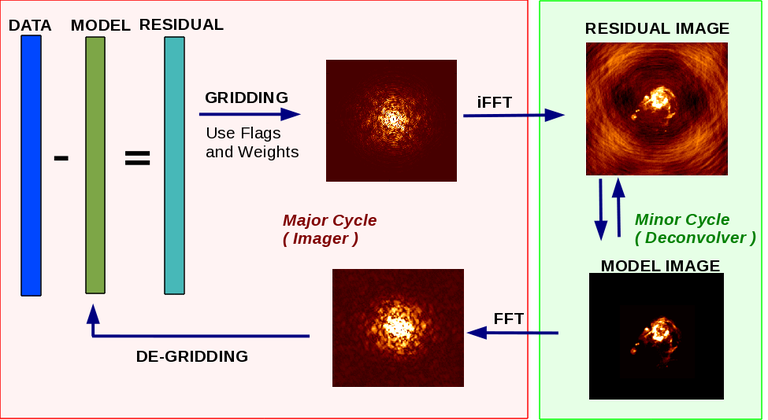
\includegraphics[width=0.9\linewidth]{./chapters/04.cs/img/casa_major_minor.png}
	\caption{Casa Major Minor Cycle. Source \cite{casa2018major}}
	\label{cs:major}
	\vspace{-10pt}
\end{wrapfigure}

CASA is a software package built for reconstructing images for VLA. 

CASA works in two separate cycles, the major and minor cycle. The major cycle transforms the Visibilities to image space and back using the Fourier Transform. The minor cycle is the deconvolution algorithm, which tries to find the true image from a dirty image and a PSF. 

The first major cycle iteration creates the PSF and the dirty image. Then, several minor cycle deconvolve the dirty image. The major cycle then continues, transforms the deconvolved image back to Visibilities. The major cycle ends by calculating the residual Visibilities from the measurement and the deconvolution. The next major cycle continues by transforming the residual Visibilities. At the end of several major cycle, the model column should contain an approximation of the true visibilities while the residuals should be noise. %it is a $\mathcal{X}^2$ approximation of the Visibilities.

In CASA the major cycle is fixed. It was evaluated if it can be modified, but a modification was too time consuming in the context of the project. However CASA allows for the addition of new deconvolution algorithms. 

Compressed Sensing Algorithm was implemented as a CASA deconvolver. The Data term of the objective is fixed to be the deconvolution ($D_{dirty} x \star PSf$). 


Major cycle is more expensive to compute than a CLEAN minor cylce. 

CLEAN needs potentially many major cycle iterations. A Compressed Sensing Reconstruction would converge to the optimum in one major cylce. Here lies a potential speedup for the Compressed Sensing Reconstruction.

%CASA is a software package built for solving the deconvolution problem for instruments like VLA and ALMA. "Data" Column measurements(calibrated), model column contains the "true" visibilities and the residual column only noise. The architecture is oriented after the CLEAN algorithm, it is split in a major and minor cycle.\ref{cs:major}. The first part of the major cycle produces the dirty image and the PSF. The minor cycle is where a deconvolution algorithm "cleans" the dirty image, several iterations of CLEAN. Major cycle ends with the forward fourier transform. Chi$^2$ approximation of the visibilities.

%The idea of the dirty beam and the clean beam. The output of CASA is the model image convolved with the clean beam plus residuals. Because the model image contains many small peaks, any structure smaller than the clean beam is implausible. Convolving with a gaussian is essentially reducing the resolution. But this is not the case. CLEAN can lead to implausible model images depending on the content: If only a few point sources are visible, clean is plausibe. But for extended emissions clean produces a an area of many peaks which is not true.. With compressed sensing, the ideal prior leads to the true model image. 

%CASA can be extended new deconvolution algorithms, changing minor cycles. During the project it was evaluated if CASA could be modified so wide Field of View imaging can handled by the minor cycle. It was not possible. The implementation is restricted to the deconvolution in the data term. This excludes the in-painting objective function. Or that the data term minimizes on the Visibilities directly.




 
